% !TEX root = ../main.tex
% Chapter Background information and theory

% \chapter{State-of-the-art of conversational agent systems} % Main chapter title
\chapter{Background information and theory} % Main chapter title

\label{Chapter2} % Change X to a consecutive number; for referencing this chapter elsewhere, use \ref{ChapterX}

A conversational agent (chatbot) is intended to respond to a Human by taking advantage of all its knowledge, its capacity to detect sentiments or remember the context, or its ability to search information on the web. Chatbots tend to use text as input and output format, but it is also possible to use speech recognition and speech generation to allow users to speak while conversing.

\section{Different approaches to building conversational agents}
Chatbots are created using two different approaches, namely the \textbf{Rule-based} approach and the \textbf{Generative} approach. The Rule-based approach, as its name indicates, uses rules to understand user input and pick from a list of answers a possible one. Rule-based chatbots exist since 1966 with the development of ELIZA chatbot in \citet{Weizenbaum:1966:ECP:365153.365168}. ELIZA's goal was to measure the psychological effects on Humans when they talk to a machine. Some of the test subjects found it really hard to believe that they were talking to a computer. ELIZA followed a script and analyzed user input to find keywords and to choose the proper answer. The workload for the developer was quite intensive and it would only take one situation that the developer might not have thought of and the user would understand he was not talking to a Human.

The Generative approach is a machine learning (ML) model that takes advantage of the recent research and technology improvements enabling deep neural networks (DNN) model to be trained on large datasets. The main difference with the rule-based approach is that the chatbot learns and establishes its own rules based on the training dataset. Thus, generative models are less entitled to misunderstand the user but since they learn themselves the output sentences, they might generate them with punctuation errors, grammatical errors, or even generate incomprehensible sentences. Besides the generation problems, training deep neural networks is not an easy task and require high-performance hardware.

These two approaches are used in two different cases, closed-domain and open-domain conversations. A closed-domain conversation means that the chatbot answers to a particular type of questions. For example, if a company develops a chatbot to let users manage their booking details, it will only be able to answer requests for bookings and nothing else. On the contrary, an open-domain chatbot is able to discuss anything. For example, Siri the personal assistant developed by Apple or Alexa the personal assistant developed by Amazon are able to understand very different requests. Figure \ref{fig:types_chatbot} shows the different types of chatbots and highlights the fact that the rule-based approach is only meant for closed-domain conversations. An open domain chatbot based on prepared scenarios and answers, following rules, is impractical due to the amount of work needed to construct such a system.

\begin{figure}
    \centering
    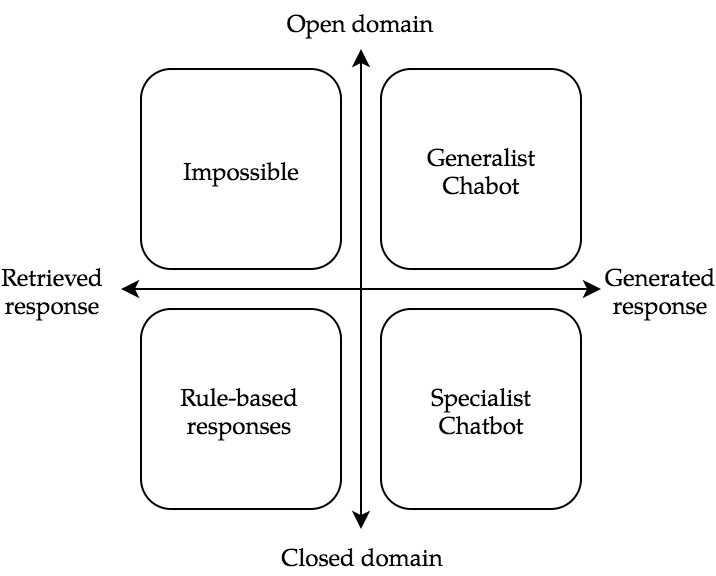
\includegraphics[width=.66\textwidth]{types_chatbot}
    \decoRule
    \caption[Different types of chatbot]{Different types of chatbot. Source: \citet{types-chatbot}.}
    \label{fig:types_chatbot}
\end{figure}

\section{Rule-based models}
In this section, two technics to build a rule-based model are presented, a markup language technic and a web-based development tool.

\subsection{Artificial Intelligence Markup Language}
Artificial Intelligence Markup Language (AIML) is an XML-compliant language that simplifies the creation of rule-based chatbots \citep{wallace2005aiml}. The four main tags are described below.
\begin{itemize}
    \item \textit{<aiml>}: tag to begin and end an AIML document
    \item \textit{<category>}: tag to create an user intent
    \item \textit{<pattern>}: each category has a pattern, which is the exact phrase the user enters in the chatbot
    \item \textit{<template>}: what the chatbot answers
\end{itemize}
An example of a category, from ALICEbot, is shown in Listing~\ref{lst:aiml}.
\begin{lstlisting}[language=XML, label={lst:aiml}]
<category>
    <pattern>WHAT ARE YOU</pattern>
    <template>
        I am the latest result in artificial intelligence,
        which can reproduce the capabilities of the human brain
        with greater speed and accuracy.
    </template>
</category>
\end{lstlisting}

\citet{wallace2009anatomy} created a chatbot of approximately 41'000 categories called ALICE. A log extract of a conversation with ALICE is shown in Listing~\ref{lst:alice-log}.
\begin{lstlisting}[label={lst:alice-log}]
judge: Hi alice
ALICE: Hi there!
judge: How are you ?
ALICE: Fair to partly cloudy.
judge: Cloudy ?
ALICE: We have never talked about it before.
judge: Who is the president of the united states ?
ALICE: Obama.
\end{lstlisting}

\subsection{Development tools for rule-based conversational agents}
The interest around chatbots has risen since March 2016, as shown Figure~\ref{fig:trend_chatbot}. Different products appeared since then on the market to help businesses and privates build and deploy chatbots. One example is Dialogflow\footnote{\url{https://dialogflow.com/}} but most of the tools follow the same logic. The goal of Dialogflow is to understand the intent of the user and to trigger an action. The action can be a text response provided by Dialogflow or, Dialogflow can use a webhook and send the intents to a remote server that builds the response accordingly to users' intents.
For example, a possible application would be a chatbot that tells a student where his next lecture is. Dialogflow understands the intent and forwards the request to the webhook. The webhook receives the intent and connects to the school servers to get the information and sends it back to the user. Figure~\ref{fig:dialogflow} shows the flow of interactions for a chatbot developed on Dialogflow.

\begin{figure}[b]
    \centering
    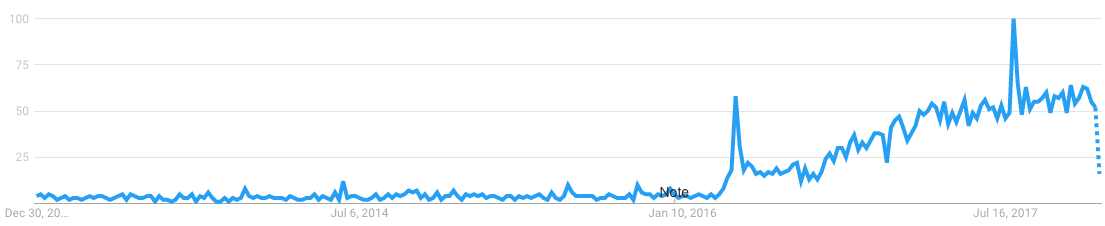
\includegraphics[width=\textwidth]{trend_chatbots}
    \decoRule
    \caption[Web search interest for ``chatbot'']{Interest of the keyword ``chatbot'' in web searches for the past 5 years. The interest suddenly rised around March 2016. Source:~Google~Trends.}
    \label{fig:trend_chatbot}
\end{figure}

\begin{figure}
    \centering
    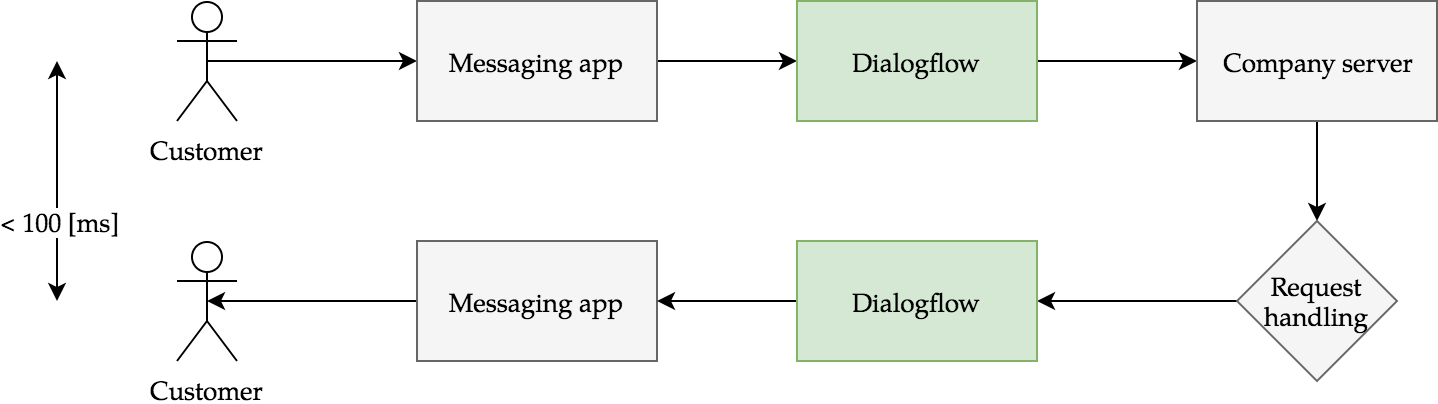
\includegraphics[width=\textwidth]{dialogflow_flow}
    \decoRule
    \caption[Dialogflow based chatbot]{Flow of interactions for a chatbot developed on Dialogflow. Since the user is speaking to a chatbot, a certain latency is acceptable but should not exceed one second.}
    \label{fig:dialogflow}
\end{figure}

The strength of these tools is that they extract the intent of the user without being restricted to an exact sentence. These tools are sometimes called hybrid because they are in their core rule-based models, but use Natural Language Processing (NLP) to understand better the user. Thus, the chatbots are more reliable and therefore, become more interesting for companies like Swiss, Comcast, The Wall Street Journal or Mercedes-Benz \citep{dialogflow}. These chatbots are deployed over popular messaging platforms like Facebook Messenger or WhatsApp. Knowing the data policy of these messaging platforms, the privacy of the data is an important concern. However, for example, Facebook's spokeswoman said that Messenger does not read the messages between people and businesses and Facebook does not use the content of Messenger conversations for any type of advertising \citep{facebook-policy}.

\section{Generative models}
Generative conversation models are based on a learning process and need a large set of training data (e.g. \citet{1506.05869} used 62M sentences). Generative models are created using deep neural networks like Recurrent Neural Network (RNN) \citep{1503.02364,1506.05869}.

\subsection{Vector representation of words}

As RNNs take real vectors as inputs, the text sequence are represented as continuous vectors, known as word embeddings. A technic called word2vec \citep{1301.3781} proposes two log-linear models based on feedforward Neural Net Language Model (NNLM) to represent efficiently words in vector space. The first model architecture of word2vec is called the Continuous Bag-of-Words (CBOW) model and follow the feedforward NNLM architecture with one hidden layer.
The idea behind is that we train a model to predict a word from a sentence using N words occurring before and N words occurring after the word in the sentence. Figure~\ref{fig:example_w2v} illustrates an example where the training sentence is \textit{``This corpus contains millions entities''} and N equals 2. Figure~\ref{fig:cbow} shows the CBOW architecture in a formal way.

\begin{figure}
    \centering
    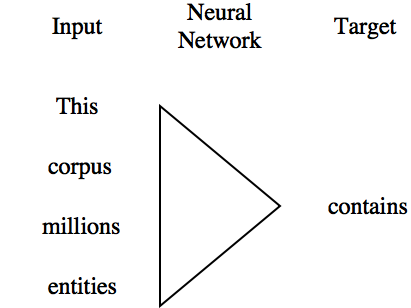
\includegraphics[width=.45\textwidth]{example_w2v}
    \caption[Word2Vec basic example]{Basic example of a training iteration in a word2vec model using the CBOW architecture. The training sentence is \textit{``This corpus contains millions entities''} and N equals 2.}
    \label{fig:example_w2v}
\end{figure}

The skip-gram architecture, represented in Figure~\ref{fig:skipgram}, takes as input the current word to predict the context. Empirical results \citep{tf.word2vec} show that the Skip-gram model is more useful for large datasets than CBOW as it fits better on small datasets.

\begin{figure}
    \centering
    \begin{subfigure}{.45\textwidth}
        \centering
        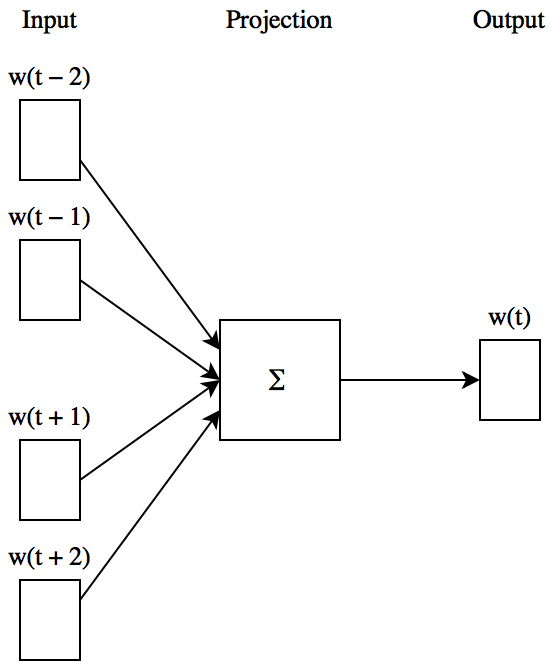
\includegraphics[width=\textwidth]{word2vec_cbow}
        \caption[Continuous Bag-of-Words architecture]{CBOW architecture from word2vec models. Context is used to predict the current word.}
        \label{fig:cbow}
    \end{subfigure}
    ~~~~~~~~~~
    \begin{subfigure}{.45\textwidth}
        \centering
        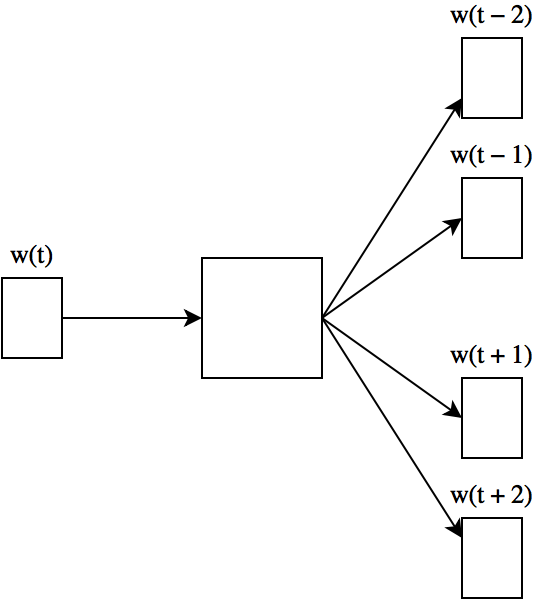
\includegraphics[width=\textwidth]{word2vec_skipgram}
        \caption[Skip-gram architecture]{Skip-gram architecture from word2vec models. Current word is used to predict the context.}
        \label{fig:skipgram}
    \end{subfigure}
    \decoRule
    \caption[Word2vec architectures]{Word2vec architectures. Source:~\citet{1301.3781}.}
    \label{fig:word2vec}
\end{figure}

An interesting finding by \citet{1301.3781} shows that simple arithmetic operations can be performed on word embeddings to highlight and find words sharing the same relation. For example, $\mathrm{queen} - \mathrm{king} + \mathrm{man} = \mathrm{woman}$.

\subsection{Recurrent Neural Networks}
RNN is a neural network created to analyze time-series. Given a sequence $\bm{x} = (x_1, ..., x_S)$, from time $t = 1$ to $S$, an RNN outputs the sequence $\bm{y} = (y_1, ..., y_T)$, iterating from time $t = 1$ to $T$.
Each RNN has two weight matrices, one for the input, $\mathbf{W}_x = (w_{ij})_x \in \mathbb{R}^{n \times m}$, $n$ being the number of features and $m$ being the number of neurons, and one for the output, $\mathbf{W}_y = (w_{ij})_y \in \mathbb{R}^{m \times m}$, as shown in Eq.~\ref{eq:rnn_y} \citep{geron2017hands}.
Let $\phi$ be an activation function and $\bm{b}$ the bias vector.

\begin{align}
    \label{eq:rnn_y}
    \bm{y}_t &= \phi (\mathbf{W}_x^T \cdot \bm{x}_t + \mathbf{W}_y^T \cdot \bm{y}_{(t-1)} + \bm{b})
\end{align}

Vanilla RNNs present two main problems, described in~\citet{bengio1994learning}, namely the exploding and the vanishing gradient problem. The exploding gradient problem means that the gradient grows exponentially to a point where the weights of the network, during the backpropagation \citep{rumelhart1986learning} are overly updated and result to a network losing all its learning. \citet{pascanu2013difficulty} proposed a simple trick to prevent exploding gradients by clipping the gradient if it becomes too big. In other words, if the gradient surpasses a certain threshold, the gradient is changed to the maximum allowed value.

The vanishing gradient problem means that the backpropagation of the gradient over the weights of the neural network has no effect on the weights themselves because the gradient is too small, meaning that the network stops learning.
Long short-term memory (LSTM) \citep{hochreiter1997lstm} is an RNN model having the capability of memorizing long distance information and being less affected by the vanishing gradient problem described in \citet{bengio1994learning}. Instead of having a single activation function, for example $\tanh$, the LSTM cell has different gates interconnected with different functions.
The following LSTM architecture is presented in \citet{1409.2329}, based on the work presented in \citet{1303.5778}. Let $\bm{h}^l_t \in \mathbb{R}^n$ be a hidden state in layer $l$ at timestep $t$ and let $T_{n,m} : \mathbb{R}^n \rightarrow \mathbb{R}^m$ be an affine transformation ($Wx + b$).
Let $\mathrm{sigm}$ be a sigmoid function, for example a $\tanh$ function and let $\odot$ be an element-wise multiplication.
Figure~\ref{fig:lstm-cell} shows a graphical illustration of an LSTM cell.

\begin{align}
    \mathrm{LSTM} &: \bm{h}_t^{l-1}, \bm{h}_{t-1}^l, \bm{c}_{t-1}^l \rightarrow \bm{h}_t^l, \bm{c}_t^l\\
    \begin{pmatrix}
        \bm{i}\\
        \bm{f}\\
        \bm{o}\\
        \bm{g}\\
    \end{pmatrix} &=
    \mathrm{sigm}
    % \begin{pmatrix}
    %     \mathrm{sigm}\\
    %     \mathrm{sigm}\\
    %     \mathrm{sigm}\\
    %     \mathrm{sigm}\\
    % \end{pmatrix}
    \ T_{2n,4n}
    \begin{pmatrix}
        \bm{h}_t^{l-1}\\
        \bm{h}_{t-1}^l\\
    \end{pmatrix} \label{equ:gates}\\
    \bm{c}_t^l &= \bm{f} \odot \bm{c}_{t-1}^l + \bm{i} \odot \bm{g} \label{equ:lstm-c}\\
    \bm{h}_t^l &= \bm{o} \odot \tanh (\bm{c}_t^l) \label{equ:lstm-h}
\end{align}

\begin{figure}
    \centering
    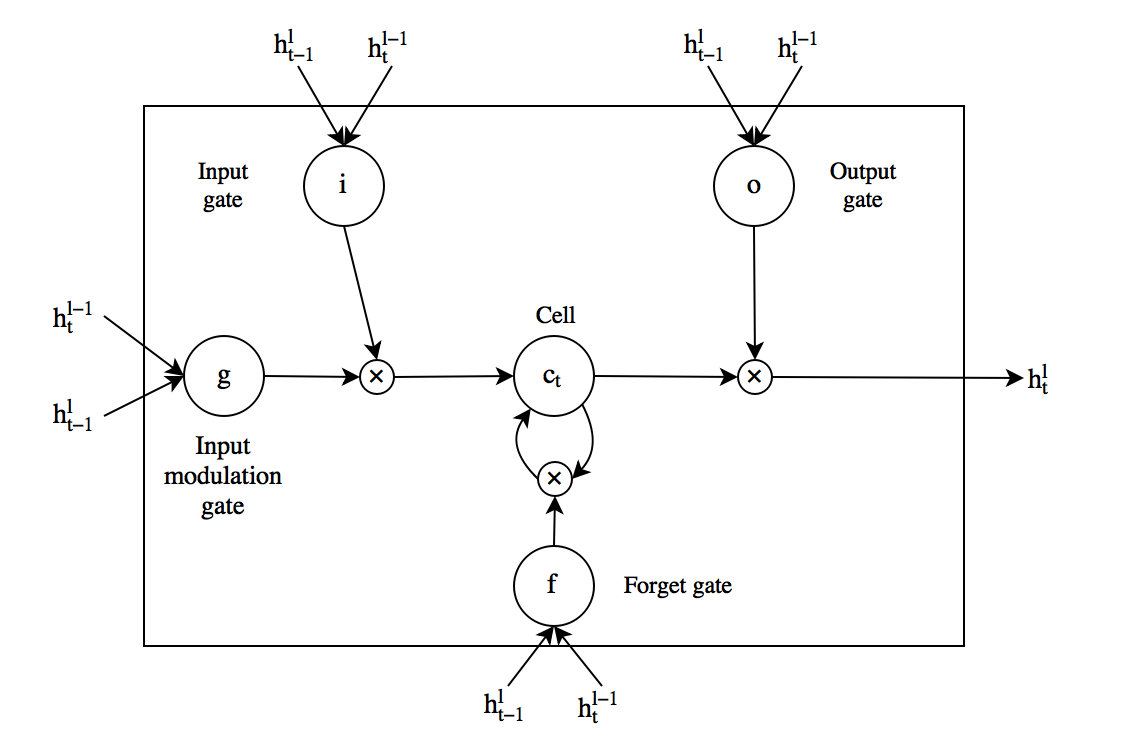
\includegraphics[width=\textwidth]{lstm_cell}
    \decoRule
    \caption[LSTM cell]{LSTM cell. Let $\bm{h}^l_t \in \mathbb{R}^n$ be a hidden state in layer $l$ in timestep $t$. Source:~\citet{1409.2329}.}
    \label{fig:lstm-cell}
\end{figure}

Dropout \citep{srivastava2014dropout} is a technic often used in neural network models to reduce the chance to overfit. The dropout randomly corrupts certain weights to force the model to learn more robustly. \citet{1409.2329} successfully applied dropout in their LSTM model by applying the dropout operator on the hidden states from the previous layer.

\subsection{Neural Machine Translation}
The Neural Machine Translation (NMT) model, proposed by~\citet{nmt-phd}, is inspired by the Sequence-to-Sequence (seq2seq) architecture. Seq2Seq) was first introduced by Google \citep{1409.3215} to be an end-to-end approach that makes only minimal assumptions on the sequence structure.
Researchers observed that building end-to-end deep learning systems based on discriminative neural networks often work better with data minimally preprocessed~\citep{chen2015handbook}.
In the use case of chatbots, the input and output sequences, or conversations, can have basically any length, only be tokenized, and the NN is able to learn. Seq2seq model takes the text as a time-series and uses RNN as the basic cell. Seq2Seq approach decomposes the architecture into two main parts, namely the encoder and the decoder. The encoder, initialized with random weights, takes as input a sequence of text and forms a fixed-size vector representation of it.
The decoder, initialized with the last hidden state of the encoder, uses this abstract representation produced by the encoder to output the adequate output sentence. The fixed-size vector representation is meant for capturing relevant information from the input sentence.
Figure~\ref{fig:seq2seqmodel} shows the seq2seq model architecture and Figure~\ref{fig:nmt} presents the workflow of an NMT model. The example shown is a translation problem, but NMT model architecture is used also for conversational agents or text summarization \citep{tensorflow.nmt}.

\begin{figure}
    \centering
    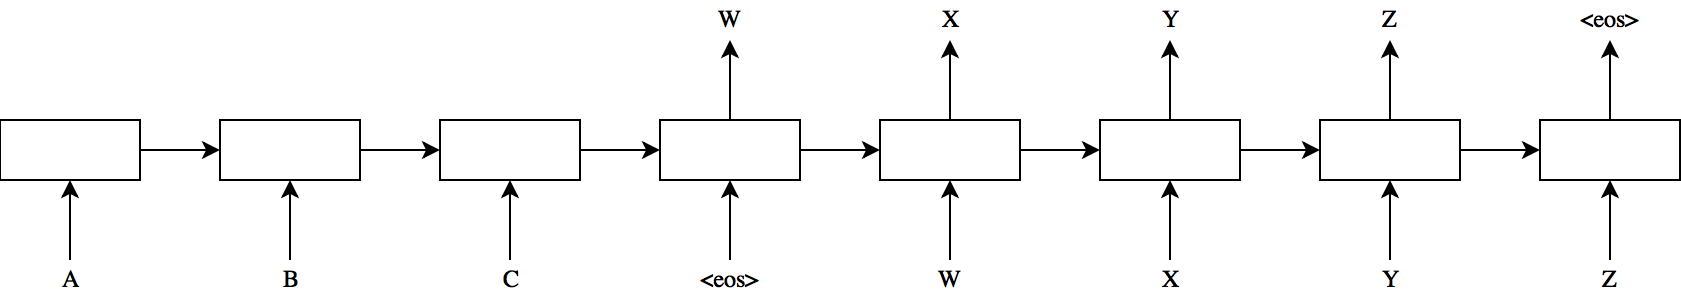
\includegraphics[width=\textwidth]{seq2seq_model}
    \decoRule
    \caption[Seq2Seq model architecture]{Seq2Seq model architecture~\citep{1409.3215}. In the decoder part of the model, the output $\bm{h}_{t-1}$ is the input $\bm{x}_{t}$.}
    \label{fig:seq2seqmodel}
\end{figure}

\begin{figure}
    \centering
    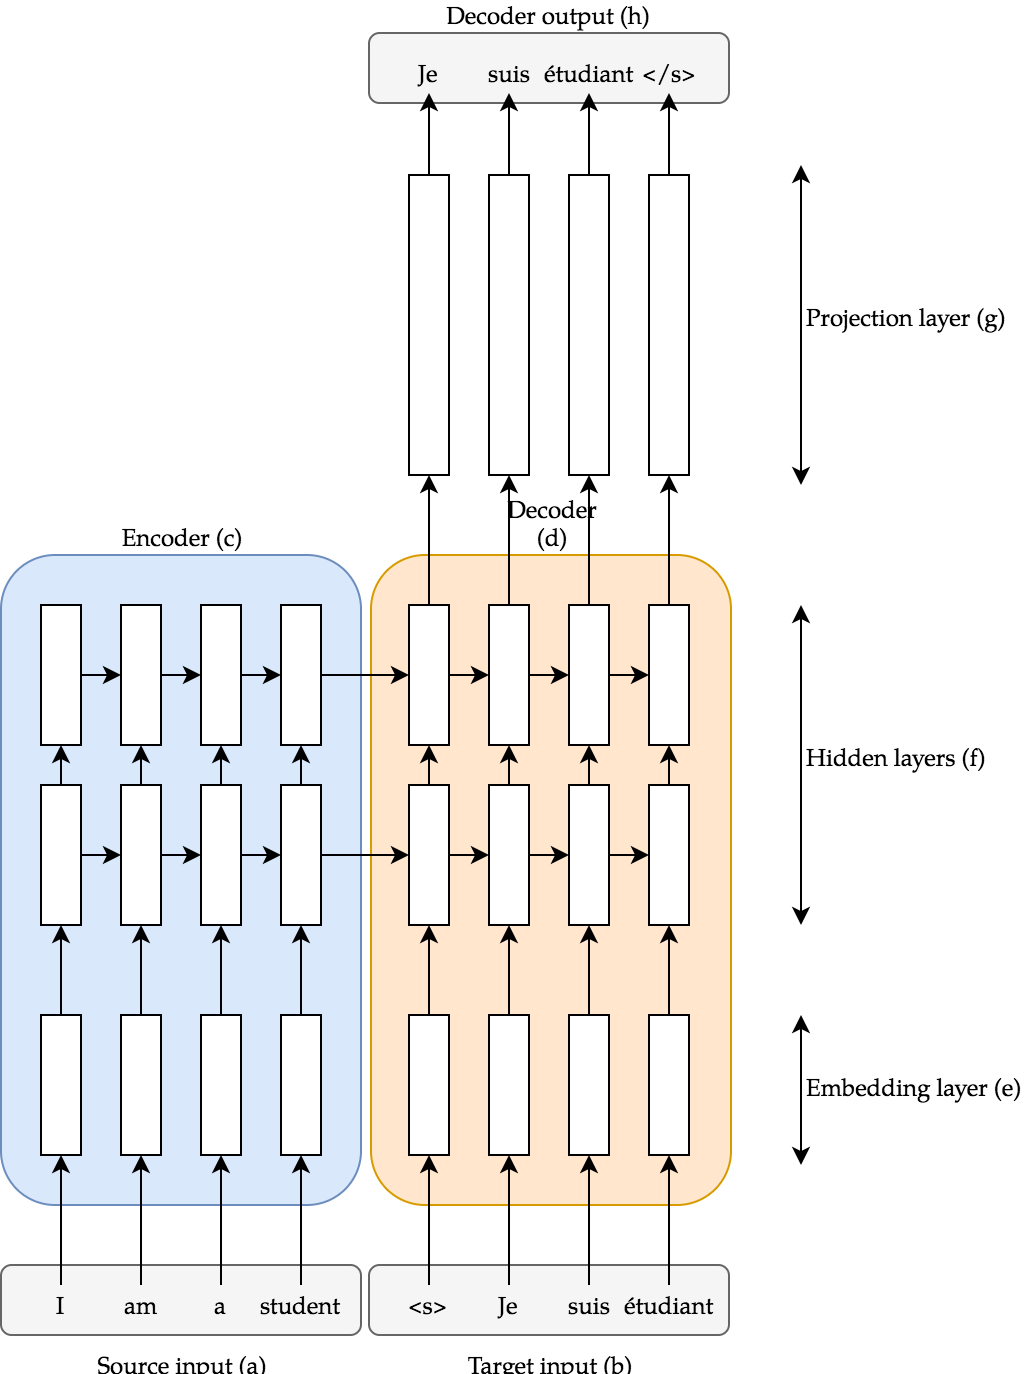
\includegraphics[width=.8\textwidth]{nmt_training_scheme}
    \decoRule
    \caption[Neural Machine Translation model scheme]{Neural Machine Translation model scheme \citep{tensorflow.nmt}. \textbf{(a)} \textit{Source input} refers to the input sequence tokenized to let the encoder read it token by token. \textbf{(b)} \textit{Target input} refers to the decoder input that lets the decoder have the correct $t-1$ token. \textbf{(c)} \textit{Embedding layer} refers to the feedforward neural network language model that creates words' vector representation. \textbf{(d)} \textit{Encoder} refers to stacked LSTMs used to build an abstract representation of the input sequence. \textbf{(e)} \textit{Decoder} refers to stacked LSTMs that produce the output sequence based on the abstract representation built by the encoder and on the previous target word. \textbf{(f)} \textit{Hidden layers} refer to the number of stacked RNN layers. \textbf{(g)} \textit{Projection layer} refers to the probability distribution of the predicted word, used to calculate the loss. \textbf{(h)} \textit{Decoder output} refers to the output sequence tokenized.}
    \label{fig:nmt}
\end{figure}

Both the encoder and the decoder are RNNs: LSTMs \citep{1409.3215,1508.04025} or GRUs \citep{1706.05125,1503.02364}. These RNN models need as input fixed-size sentences but conversations have varying length. To face this issue, the sentences are padded with $0$ vectors to reach the size of the longest sentence of the training set. However, a lot of computation and memory is required to save vectors filled with zeros and train a model. This computation leak is resolved by bucketing the training set based on the length of the sentence.
Bucketing means that the training set is partitioned into buckets containing sentences of approximately the same length. With buckets, sentences are still zero padded to the longest sentence of the bucket but it ensures that the padding is minimized.

% \textbf{Calculate the number of parameters}

% \textbf{Evaluation: loss, perplexity, cross-entropy, BLEU, being an active research topic today}
The top layer of the decoder is fed to a softmax function to produce the predictive distribution. This distribution is used to extract the probability of every word being the target word or not, then the most probable word is chosen and output. To know how good a model works, the categorical cross-entropy is calculated between the target and decoded distribution and used as the loss function to backpropagate the error through the network.

Perplexity (PP) is a metric used to evaluate language models, instead of using raw probabilites. As described in~\citet{jurafsky2014speech}, the perplexity of a language model on a test set is \textit{the inverse probability of the test set, normalized by the number of words}. Let $\mathbf{W}$ be a test set $\mathbf{W}=w_1 w_2 ... w_N$ and let $N$ be the size of the test set. Equation~\ref{equ:pp} defined the perplexity.
PP is normalized over the length sentences because the longer the sentence, the less proabable it is going to be, so the normalization allows the measure to be possible over multiple lengths sentences \citep{nlp-jurasky-4.4}.
In other words, minimizing the perplexity is the same as maximizing the probability, the probability of having a word after a prefix sequence.

\begin{equation}
    \mathrm{PP}(\mathbf{W}) = \sqrt[N]{ \prod_{i=1}^N \frac{1}{P(w_i | w_1 ... w_{i-1})}  }
    \label{equ:pp}
\end{equation}

Moreover, to measure how good a model actually generates words, the BLEU score, \citet{bleu-score}, is used. As opposed to the perplexity being an intrisic evaluation metric, the BLEU score is an extrinsic evaluation. The BLEU score measures the closeness of words between the decoded and target sentences using an n-gram precision.
% \begin{equation}
%     \mathrm{BLEU} = XX, \mathrm{BLEU} \in [0, 100]
%     \label{equ:bleu}
% \end{equation}
In NMT, the BLEU score works well because a translation is often the same even with a different context. For example, ``maison'' in French will almost always be translated as ``house'' in English.
However, when dealing with conversational agents, the context can vary a lot, from the way the user write to, for example, the weather. From this observation, \citet{1603.08023} showed that there is not currently a reliable method to measure the effectiveness of a chatbot, except the use of Human evaluators.

Once the model is trained, there are mainly two approaches to decode a sentence, known as inference, namely the greedy search or the beam search. The greedy search takes the most probable output word at each timestep and fed it in the decoder's input at $t+1$. This approach is computationally efficient but does not yield great quality. Figure~\ref{fig:nmt-inference} shows the inference process using a greedy search.
\begin{figure}
    \centering
    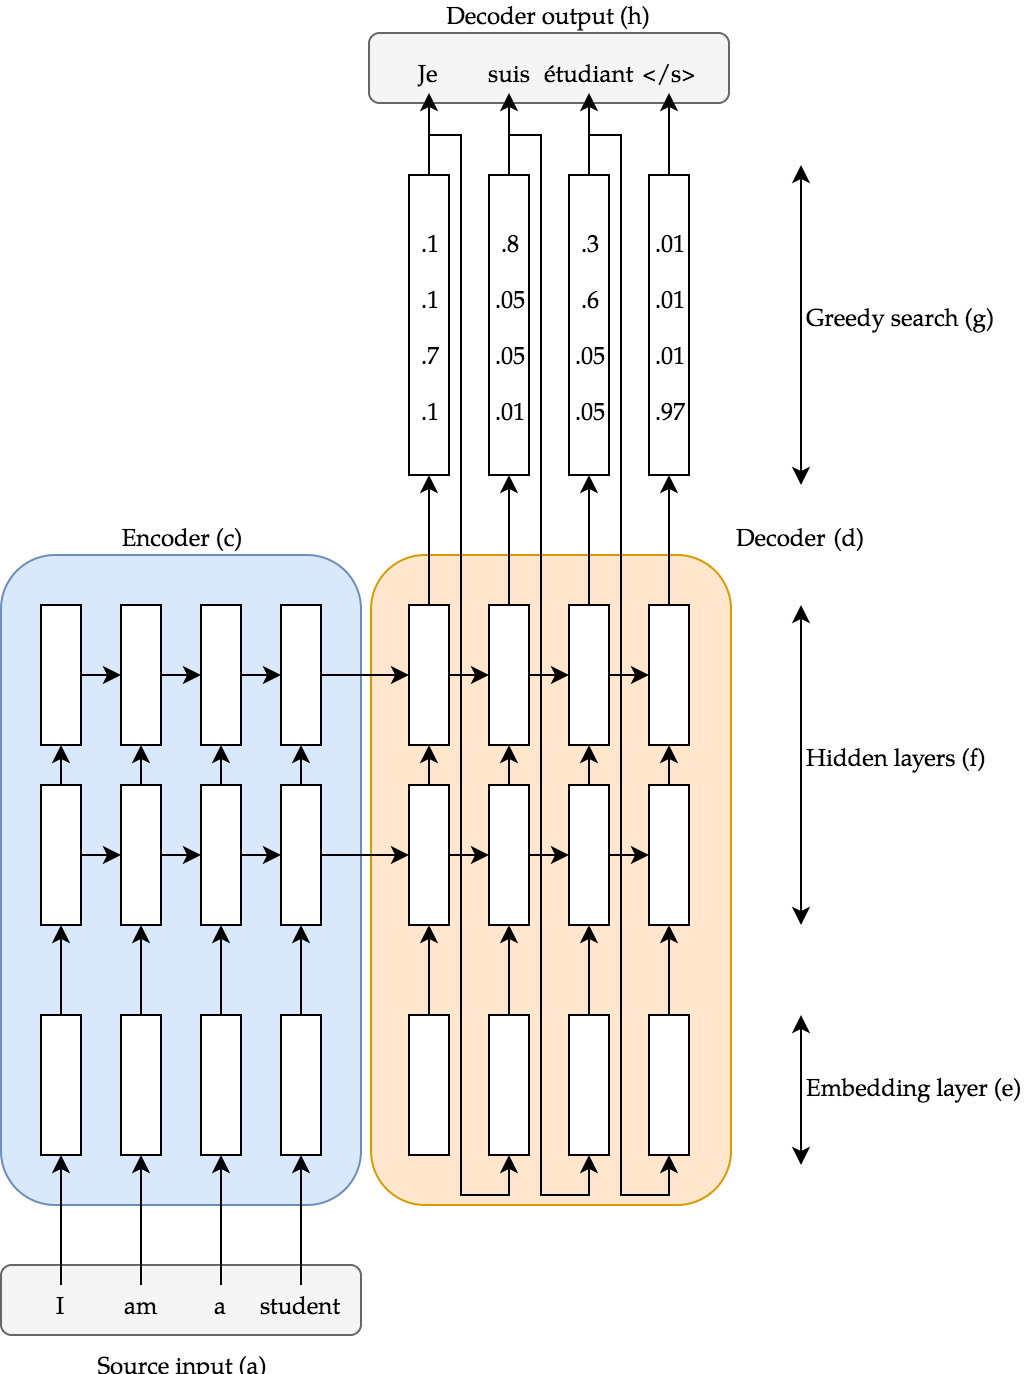
\includegraphics[width=.8\textwidth]{nmt_inference_scheme}
    \decoRule
    \caption[Neural Machine Translation inference scheme]{Neural Machine Translation inference \citep{tensorflow.nmt}. \textbf{(a)} \textit{Source input} refers to the input sequence tokenized to let the encoder read it token by token. \textbf{(b)} \textit{Embedding layer} refers to the feedforward neural network language model that creates words' vector representation. \textbf{(c)} \textit{Encoder} refers to stacked LSTMs used to build an abstract representation of the input sequence. \textbf{(d)} \textit{Decoder} refers to stacked LSTMs that produce the output sequence based on the abstract representation built by the encoder and on the $t-1$ output word. \textbf{(e)} \textit{Hidden layers} refer to the number of stacked RNN layers. \textbf{(f)} The \textit{Greedy search} takes the most probable output word at each timestep  \textbf{(g)} \textit{Decoder output} refers to the output sequence tokenized.}
    \label{fig:nmt-inference}
\end{figure}

The beam search is computationally more expensive than the greedy search but yields much better quality. The process of the beam search is to keep track of the most probable words at each timestep and to feed the decoder's input with the N most probable words until the number of possibilities excess a certain threshold. At each time, the probability of the whole sequence is calculated and only the words being in the most probable sentence are kept for $t+1$.


\subsection{Attention mechanism}
Intuitively, when one translates a sentence, one does not only read the sentence once and straightly translates it. The translation is based on the sentence overall, the translator goes back and forth in the source sentence to give the proper translation. The same intuition applies to conversations.
In basic seq2seq architecture, the model only bases its input data knowledge on the encoder's last hidden state. \citet{1508.04025} proposed a simple method to allow the model to pay attention to what matters at every timestep. They based their work on the research conducted by \citet{1409.0473} that proposed an improvement in seq2seq model performance by allowing ``\textit{the model to automatically (soft)-search for parts of a source sentence that are relevant to predicting a target word}''.

\begin{figure}
    \centering
    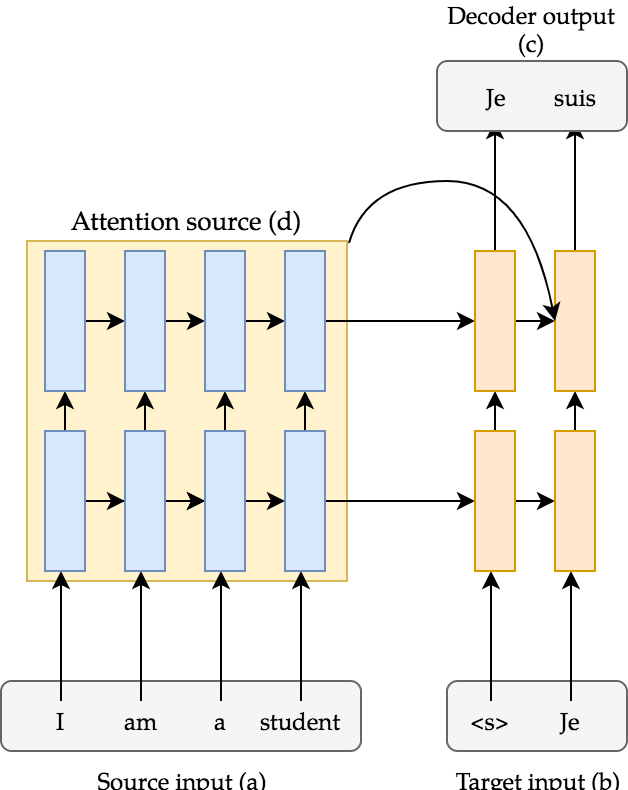
\includegraphics[width=.6\textwidth]{attention_basic_scheme}
    \decoRule
    \caption[Attention basic scheme]{Attention basic scheme. The decoder uses what is relevant from the input source to decode the sentence and not only the last hidden state of the encoder. Source:~\citet{youtube-nmt-attention}.}
    \label{fig:attention_basic_scheme}
\end{figure}

The attention mechanism can be seen as a memory which the model retrieves information when needed. Figure~\ref{fig:attention_basic_scheme} shows the decoder taking into account attention in the decoding process.
\citet{1508.04025} proposed a simple and effective approach of the attention mechanism separated into two models, namely the \textit{global attention} and \textit{local attention}, following nevertheless a common ground.
At each time step $t$, the hidden-state $\bm{h}_t$ at the top layer of the stacked LSTMs is given as input of the attention layer.
The goal is to construct a context vector $\bm{c}_t$ that captures relevant source-side information that helps to predict the current target word $\bm{y}_t$. As for the basic NMT model, the decoder output is sent to a softmax function to calculate the probability distribution.
In an attention-based NMT, the current target hidden state $\bm{h}_t$ is concatenated with the context vector $\bm{c}_t$ to produce an attentional hidden state $\bm{\tilde{h}_t}$, as showed in Eq.~\ref{equ:atn-hidden-state}. Let $\mathbf{W}_c$ be the weight matrix parametrizing the construction of $\bm{\tilde{h}_t}$.
Then, $\bm{\tilde{h}_t}$ is fed through the softmax layer, as showed in Eq.~\ref{equ:atn-hidden-state-to-softmax}.
\begin{equation}
    \bm{\tilde{h}}_t = \tanh ( \mathbf{W}_c [\bm{c}_t;\bm{h}_t])
    \label{equ:atn-hidden-state}
\end{equation}
\begin{equation}
    p( \bm{y}_t | \bm{y}_{<t}, \bm{x}) = \mathrm{softmax}(\mathbf{W}_s \bm{\tilde{h}}_t)
    \label{equ:atn-hidden-state-to-softmax}
\end{equation}
 The global and local attention models differ on how the context vector $\bm{c}_t$ is derived.

 The global attentional model takes into account all the hidden states of the decoder's top layer to produce the context vector $\bm{c}_t$. This model compares the current target hidden $\bm{h}_t$ with each source hidden state $\bm{\bar{h}}_s$ to derive a variable-length alignment vector $\bm{a}_t$ whose size equals the number of time steps on the source side.
 $\bm{c}_t$ is then computed as the weighted average over all source states.
 \begin{align}
    \bm{a}_t(s) &= \mathrm{align}(\bm{h}_t, \bm{\bar{h}}_s)\\
    \label{equ:atn-a_t}
    &= \frac{\mathrm{exp}(\mathrm{score}(\bm{h}_t, \bm{\bar{h}}_s))}{\sum_{s'} \mathrm{exp}(\mathrm{score}(\bm{h}_t, \bm{\bar{h}}_{s'}))}
 \end{align}
The score function $\mathrm{score}(\bm{h}_t, \bm{\bar{h}}_s)$ is presented in three different alternatives in~\citet{1508.04025}, as described in Eq.~\ref{equ:atn-score}.
\begin{subequations}
    \label{equ:atn-score}
    \begin{align}[left ={\mathrm{score}(\bm{h}_t, \bm{\bar{h}}_s) = \empheqlbrace}]
        & \bm{h}_t^T \bm{\bar{h}}_s & \mathit{dot} \label{equ:atn-score-dot}\\
        & \bm{h}_t^T \mathbf{W}_a \bm{\bar{h}}_s & \mathit{general} \label{equ:atn-score-general}\\
        & \bm{v}_a^T \tanh ( \mathbf{W_a} [\bm{h_t}^T;\bm{\bar{h}}_s]) & \mathit{concat} \label{equ:atn-score-concat}
    \end{align}
\end{subequations}
The first alternative of the score function is described in Eq.~\ref{equ:atn-score-dot} and simply performs a dot product between the decoder hidden state and encoder hidden state and tries to find the words that are similar.
The score function described in Eq.~\ref{equ:atn-score-general} resembles the ``\textit{dot}'' score function but instead, places a weight matrix in-between to let the model parametrize the dot product, and thus capture what part of the hidden states are relevant. \citet{youtube-nmt-attention} highlights the \textit{``general''} approach to work better than the two others and being the form well-adopted by the community.
The last alternative of the score function, described in Eq.~\ref{equ:atn-score-concat}, is the one proposed by \citet{1409.0473}. In this situation, the score function is like a neural network layer and the decoder and encoder hidden states are concatenated together, then multiplied by a weight matrix, fed to a sigmoid function and finally multiplied by a vector. The main concern with the last alternative is that the two hidden states are not interacting with each other.

\citet{1508.04025} approach is similar to \citet{1409.0473} but they have three main differences that simplify and generalize the concept. First, in \citet{1409.0473}, instead of using only the top hidden states, the model concatenates all source hidden states of the bidirectional encoder to the target hidden states.
Secondly, \citet{1409.0473} computation path requires hidden states from previous time whereas in \citet{1508.04025}, only the current time hidden states are used. Finally, as mentioned before, \citet{1409.0473} used the third function score, described in Eq.~\ref{equ:atn-score-concat}.
Figure~\ref{fig:atn_global} shows the global attention model.

\begin{figure}
    \centering
    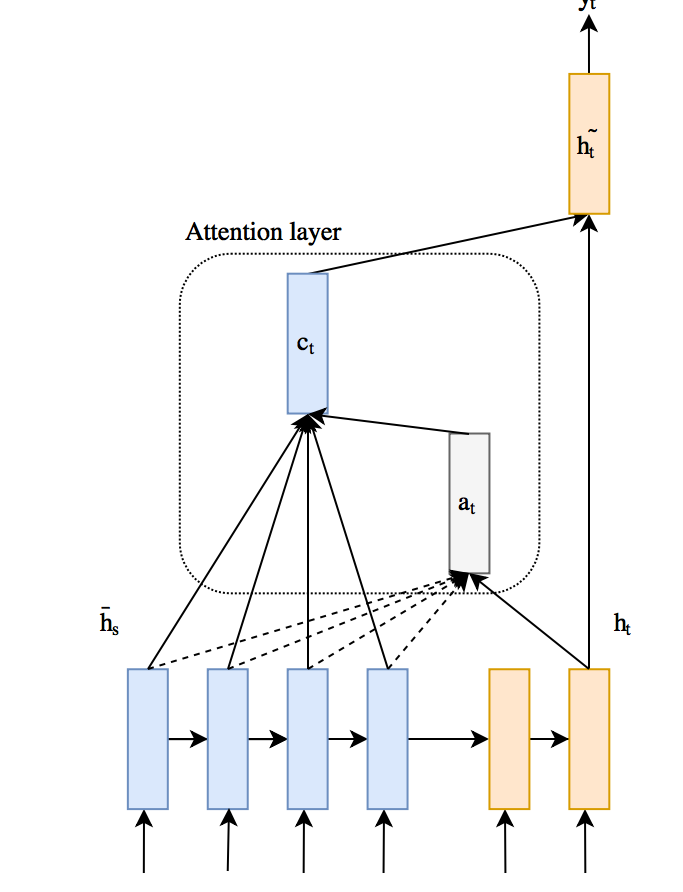
\includegraphics[width=.6\textwidth]{atn_global}
    \decoRule
    \caption[Global attention model]{Global attention model. At each time step $t$, the model derives an alignment vector $\bm{a}_t$ by comparing the source hidden states $\bm{\bar{h}}_s$ and the current target state $\bm{h}_t$ with a score function. Context vector $\bm{c}_t$ is then computed as the weighted average, according to $\bm{a}_t$, over all source states. Source:~\citet{1508.04025}.}
    \label{fig:atn_global}
\end{figure}

The local attentional model, proposed by \citet{1508.04025}, uses only a certain window around a position to compute the context vector. In other terms, it does not focus on everything at each timestep. In comparison to the global attentional model, the local attentional model is less expensive since it chooses the subset of the source positions per target word. At each timestep $t$, the context vector is created as a weighted average over the set of source hidden states within the window $[p_t - D, p_t + D]$, $D$ being empirically chosen.
This window allows the attentional vector $\bm{a}_t$ to have a fixed size $(\bm{a}_t \in \mathbb{R}^{2D+1})$. The $p_t$ parameter can be set by two different alignment methods. The \textit{monotonic alignment} simply sets $p_t = t$, assuming the source and the target sequences are somewhat aligned. The \textit{predictive alignment} learns and predicts $p_t$ in a form of a single layer feedforward neural network, as shown in Eq.~\ref{equ:atn-pt-local-align}, $S$ being the sentence length, $\mathbf{W}_p$ being the network weights matrix.
\begin{equation}
    p_t = S \cdot \mathrm{sigmoid} ( \bm{v}_p^T \tanh ( \mathbf{W}_p \bm{h}_t))
    \label{equ:atn-pt-local-align}
\end{equation}
The position $p_t$ is taking into account to construct the alignment vector $\bm{a}_t(s)$ as defined in Eq.~\ref{equ:atn-at-pt}, the standard deviation being empirically set as $\sigma = \frac{D}{2}$.
\begin{equation}
    \bm{a}_t(s) = \mathrm{align}(\bm{h}_t, \bm{\bar{h}}_s) \ \mathrm{exp}(- \frac{(s - p_t)^2}{2\sigma^2})
    \label{equ:atn-at-pt}
\end{equation}
Figure~\ref{fig:atn-local} shows the local attention model.
\begin{figure}
    \centering
    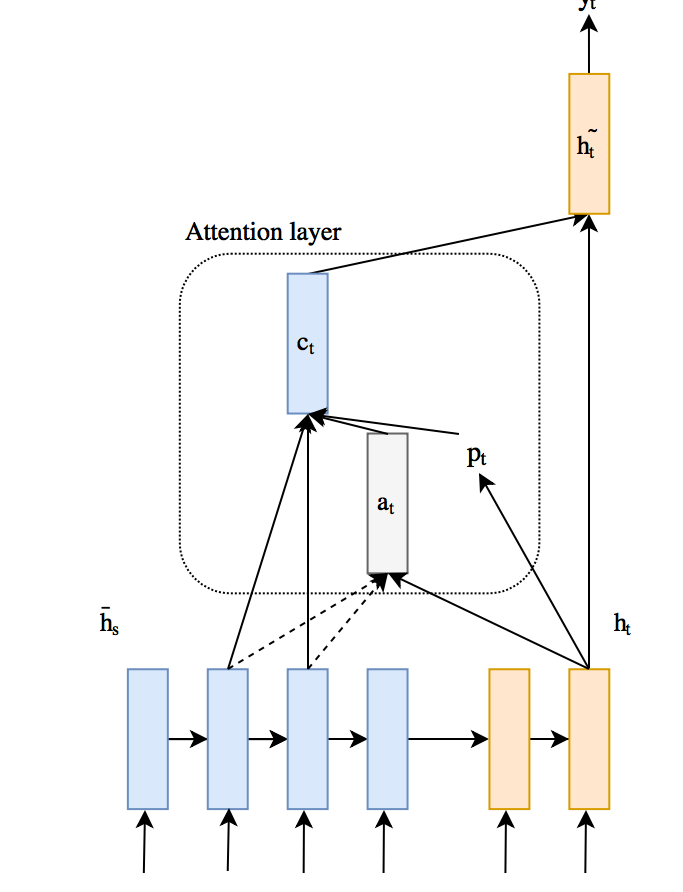
\includegraphics[width=.6\textwidth]{atn_local}
    \decoRule
    \caption[Local attention model]{Local attention model using predictive alignment. The alignment vector $\bm{a}_t$ is inferred from a selected window of hidden states $\bm{\bar{h}}_s$. The position $p_t$ is learned and predicted to have a better alignment between the source hidden states $\bm{\bar{h}}_s$ and the current target state $\bm{h}_t$. Source:~\citet{1508.04025}.}
    \label{fig:atn-local}
\end{figure}

\section{Advanced conversational agents}
Despite the fact that NMT can be used as an architecture for chatbots, more advanced models use other components that empower the chatbot with more capabilities like sentiment analysis or information retrieval.

\subsection{Emotional conversational agents}
Chatbots are interesting to discuss with and sometimes they are useful, but in certain domain, like psychology, being able to react sentimentally according to user's feelings can improve user experience and accomplish the awaited result. \citet{ecm-1704.01074} proposed an ``\textit{end-to-end framework to incorporate emotion influence in large-scale conversation generation}'' called the Emotional Chatting Machine (ECM). The model baseline is the same as the NMT model augmented with the attention mechanism, but ECM incorporates additionally two memory layers, an internal and an external memory, and an emotion embedding.

ECM integrates six different emotions categories, namely \textit{Anger, Disgust, Happiness, Like, Sadness, Other}. Instead of creating a chatbot capable of choosing the appropriate emotion category to generate a response, \citet{ecm-1704.01074} simplified and focused the problem by generating a different response for every emotion category. Table~\ref{tab:ecm} shows an example of different answers for a particular post.

\begin{table}
    \caption[Emotional chatting machine sample responses]{Emotional chatting machine sample responses. Source:~\citet{ecm-1704.01074}.}
    \label{tab:ecm}
    \centering
    \begin{tabularx}{\textwidth}{X | l | p{5cm}}
        \toprule
        \tabhead{Post} & \tabhead{Emotion Category} & \tabhead{Response}\\
        \midrule
        % \cmidrule(lr){4-1}
        \multirow{5}{4cm}{Knowing the truth, I laughed myself to tears} & Like & Too lovely it's too lovely. \\
        & Happiness & I can't help laugh myself to tears. \\
        & Sadness & After knowing the truth, I burst into tears. \\
        & Disgust & Is this true? \\
        & Anger & What do you mean? I don't understand.\\
        \bottomrule
    \end{tabularx}
\end{table}

\subsection{MILABOT for Amazon Alexa Prize Competition}
Open domain chatbots trained using machine learning algorithms without hand-crafted rules is an ongoing research topic. On this basis, Amazon.com launched in 2016 the Amazon Alexa Prize Competition with the goal of building a socialbot, in other terms, a chatbot being able to discuss nearly anything (e.g. sports, entertainment, politics). \citet{alexa-1709.02349} presented the best chatbot, called MILABOT, capable of having a conversation to about 14 to 16 turns (i.e. a turn is an answer from the user or the chatbot).
MILABOT is an ensemble-based machine learning system. It has several components that are trained to answer particular questions scored with an internal confidence. All the confidence score of all the modules are evaluated by the dialogue manager to output the most appropriate answer. Figure~\ref{fig:milabot-flow} shows the dialogue manager control flow.

\begin{figure}
    \centering
    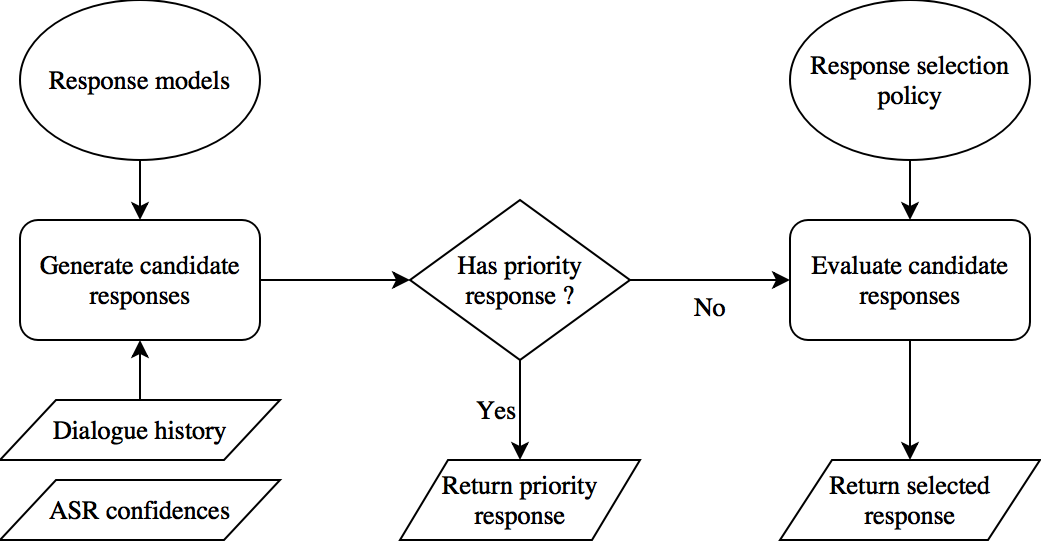
\includegraphics[width=.8\textwidth]{milabot_flow}
    \decoRule
    \caption[MILABOT dialogue manager control flow]{MILABOT dialogue manager control flow. The different modules generate their response with a confidence score. Then, the dialogue manager evaluates the different confidence scores and output the most appropriate response. Source:~\citet{alexa-1709.02349}.}
    \label{fig:milabot-flow}
\end{figure}
